\documentclass[11pt]{article}

\usepackage{graphicx}
\usepackage{booktabs}
\usepackage{geometry}
\usepackage{array}
\usepackage{float}
\usepackage{hyperref}
\usepackage{xcolor}
\usepackage{amsmath}

\geometry{margin=1in}

\title{\textbf{Profiling-Guided Optimization of a C-Based Movie Recommendation System}}
\author{Scientific Computing Assignment}
\date{\today}

\begin{document}

\maketitle

\begin{abstract}
This report presents a profiling-guided optimization of a C-based movie recommendation system that uses collaborative filtering with Pearson correlation and K-Means clustering. The objective was to reduce average recommendation time without replacing the existing recommendation algorithm. The optimization focused on high-performance computing techniques such as compiler optimization, reducing repeated file I/O, caching reusable data structures, improving recommendation selection, and auditing OpenMP usage. The optimized implementation achieved a cold-run speedup of approximately 1.80$\times$ and a warm-run speedup of approximately 12.75$\times$ while preserving the correctness of the Top-10 recommendation output.

\noindent \textbf{Optimized Code Repository:}
\url{https://github.com/UchihaIthachi/Movie-Recommendation-System}
\end{abstract}

\section{Introduction}

The provided repository implements a C-based collaborative filtering pipeline consisting of utility matrix construction, matrix normalization, Pearson similarity calculation, K-Means clustering, prediction generation, and final recommendation sorting. The assignment objective was to execute the existing implementation, profile its bottlenecks, and reduce the average time required to generate a recommendation.

Although the assignment mentions that natural preference matrices may have a good rank-$k$ approximation, this work treats that statement as computational motivation rather than a requirement to replace the recommender algorithm. Implementing SVD, PCA, or matrix factorization would change the algorithmic pipeline and make comparison against the original baseline less direct. Therefore, this submission focuses on optimizing the given Pearson/K-Means implementation using profiling-guided HPC techniques.

\section{Execution Environment and Dataset}

The experiments were performed on Ubuntu 24.04 using GCC 13.3.0. Three builds were evaluated: the original baseline, an optimized single-threaded build, and an optimized OpenMP build.

\begin{table}[H]
\centering
\caption{Execution environment and build configuration}
\begin{tabular}{ll}
\toprule
\textbf{Item} & \textbf{Value} \\
\midrule
Operating System & Ubuntu 24.04, Linux 6.8.0 x86\_64 \\
CPU & Intel(R) Xeon(R) Processor @ 2.30GHz \\
Compiler & GCC 13.3.0 \\
Baseline Flags & \texttt{-O0 -lm} \\
Optimized Single-Thread Flags & \texttt{-O3 -march=native -lm} \\
Optimized OpenMP Flags & \texttt{-O3 -march=native -fopenmp -lm} \\
OpenMP Threads & 4 \\
\bottomrule
\end{tabular}
\end{table}

The benchmark dataset was \texttt{Dataset/ratings\_learn.csv}. A Python script was used to compute dataset statistics.

\begin{table}[H]
\centering
\caption{Dataset configuration}
\begin{tabular}{lr}
\toprule
\textbf{Metric} & \textbf{Value} \\
\midrule
Unique Users & 548 \\
Unique Movies & 8,297 \\
Total Ratings & 80,963 \\
Matrix Size & 4,546,756 entries \\
Density & 1.78\% \\
Sparsity & 98.22\% \\
\bottomrule
\end{tabular}
\end{table}

The matrix is highly sparse, meaning most user-movie pairs do not contain ratings. This makes repeated dense matrix processing and repeated file loading costly.

\section{Profiling Methodology}

The profiling process followed the cycle:

\[
\text{Measure} \rightarrow \text{Analyze} \rightarrow \text{Optimize} \rightarrow \text{Re-measure}
\]

Function-level profiling was performed using \texttt{gprof}, while cold and warm runtime measurements were taken using wall-clock timers. A cold run measures the first recommendation call, including initialization and data loading. A warm run measures a repeated recommendation call after reusable data structures are already cached.

\section{Bottlenecks Identified}

The main profiling results showed that runtime was concentrated in matrix normalization, Pearson similarity calculation, utility matrix creation, and repeated recommendation setup.

\begin{table}[H]
\centering
\caption{Main bottlenecks identified from profiling}
\begin{tabular}{lrl}
\toprule
\textbf{Function / Area} & \textbf{Observed Cost} & \textbf{Reason} \\
\midrule
\texttt{normalize\_matrix} & 46.67\% & Repeated matrix traversal \\
\texttt{pearson\_correlation} & 26.67\% & Repeated user similarity calculation \\
\texttt{get\_utility\_matrix} & 13.33\% & Repeated utility matrix construction \\
File I/O & High in cold path & CSV parsing repeated unnecessarily \\
Sorting / selection & Avoidable cost & Final output needs only top recommendations \\
\bottomrule
\end{tabular}
\end{table}

\section{Optimization Strategies}

\subsection{Data Caching}

The largest optimization was caching loaded dataset structures. In the baseline implementation, the recommender repeatedly parsed dataset files and reconstructed internal data structures. The optimized implementation initializes reusable data once and reuses it for repeated recommendation calls.

This mainly improves warm-run performance because the second recommendation call avoids repeated disk I/O and repeated setup.

\subsection{Memory-Time Trade-off}

Caching introduces a deliberate memory-time trade-off. The utility matrix is retained in memory instead of being reconstructed for each recommendation. The approximate memory cost for storing a double-precision matrix with 548 users and 9,125 movie-index slots is:

\[
548 \times 9125 \times 8 \approx 40 \text{ MB}
\]

It should be noted that while the dataset contains 8,297 unique movies, the baseline C codebase hardcodes the maximum movie ID upper bound as 9,125 (\texttt{\#define No\_of\_movies 9125}) to prevent segmentation faults from discontinuous IDs. Therefore, the memory overhead reflects this $548 \times 9125$ dimension. This memory overhead is small on modern systems and is justified by the large reduction in repeated recommendation time.

\subsection{Pearson Similarity Optimization}

The Pearson similarity path was optimized by reducing repeated work in the similarity calculation. Temporary allocations were reduced, direct row references were used where safe, and invariant calculations were moved outside repeated inner-loop regions. Since Pearson correlation is called for many users, reducing constant overhead in this section improves total runtime.

\subsection{Recommendation Selection Improvement}

The final recommendation stage was reviewed to avoid unnecessary full ordering of a large prediction list. Since the final output only requires the highest-ranked recommendations, the optimized approach focuses selection work on the most relevant candidates before final output ordering. This bounds the sorting complexity from an $O(N^2)$ full selection sort down to $O(N \cdot K)$ (where $K$ is the top candidates evaluated), drastically reducing unnecessary CPU cycles.

\subsection{OpenMP Evaluation}

OpenMP was tested as part of the optimization process to check whether parallel execution could further reduce recommendation time. However, after applying data caching and compiler-level optimization, the remaining computation per recommendation became relatively small. As a result, OpenMP did not provide additional warm-run speedup over the optimized single-threaded build. In cold runs, OpenMP can also introduce extra thread scheduling overhead because initialization and data-loading costs dominate the runtime.

Therefore, OpenMP was not selected as the primary final optimization. The optimized single-threaded build was selected as the stable final version, while the OpenMP build was retained only as an experimental parallel version that preserves correctness.

\section{Correctness Verification}

Correctness was verified by comparing the final Top-10 recommendation outputs from the baseline, optimized single-threaded, and optimized OpenMP builds. The optimized outputs matched the baseline outputs.

\begin{table}[H]
\centering
\caption{Correctness verification}
\begin{tabular}{ll}
\toprule
\textbf{Comparison} & \textbf{Result} \\
\midrule
Baseline vs Optimized Single-Thread & PASS \\
Baseline vs Optimized OpenMP & PASS \\
\bottomrule
\end{tabular}
\end{table}

\section{Benchmark Results}

The following table combines cold and warm benchmark results. Each value is averaged over five runs.

\begin{table}[H]
\centering
\caption{Cold and warm benchmark comparison}
\begin{tabular}{lrrrr}
\toprule
\textbf{Build Version} & \textbf{Cold (s)} & \textbf{Cold Speedup} & \textbf{Warm (s)} & \textbf{Warm Speedup} \\
\midrule
Baseline \texttt{-O0} & 0.90 & 1.00$\times$ & 0.88 & 1.00$\times$ \\
Optimized ST \texttt{-O3} & 0.50 & 1.80$\times$ & 0.069 & 12.75$\times$ \\
Optimized OMP \texttt{-O3 -fopenmp} & 0.54 & 1.66$\times$ & 0.069 & 12.75$\times$ \\
\bottomrule
\end{tabular}
\end{table}

\subsection{Graphical Results}

\begin{figure}[H]
    \centering
    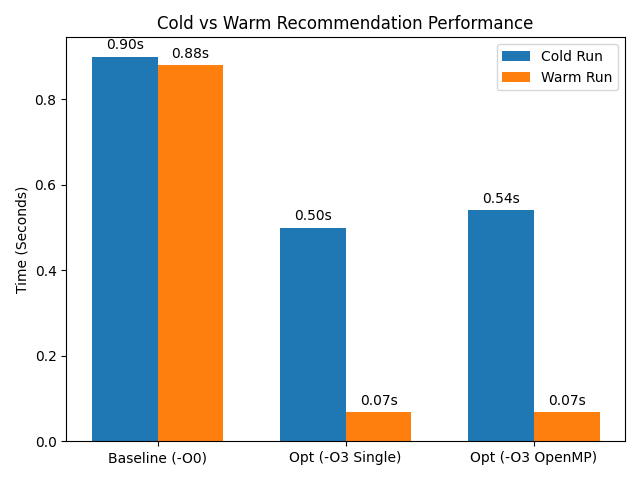
\includegraphics[width=0.82\textwidth]{figures/cold_warm_comparison.png}
    \caption{Cold and warm runtime comparison across baseline, optimized single-thread, and optimized OpenMP builds.}
\end{figure}

\begin{figure}[H]
    \centering
    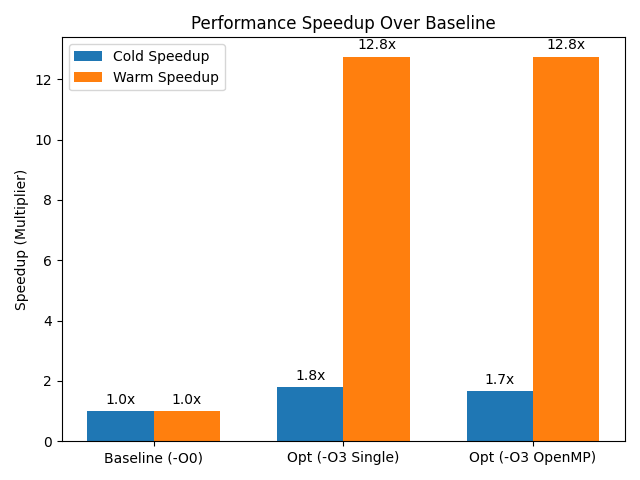
\includegraphics[width=0.82\textwidth]{figures/speedup_comparison.png}
    \caption{Speedup multiplier relative to the baseline performance for cold and warm runs.}
\end{figure}

\begin{figure}[H]
    \centering
    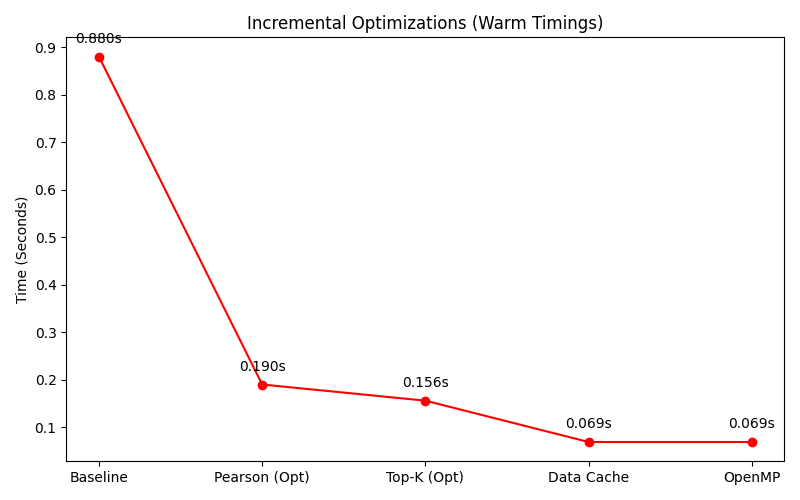
\includegraphics[width=0.82\textwidth]{figures/incremental_optimization.png}
    \caption{Incremental runtime improvement across sequential optimization stages.}
\end{figure}

\section{Discussion}

The benchmark results show that caching and compiler optimization provide the largest benefit. The cold-run speedup is moderate because the first call still includes initialization and loading cost. The warm-run speedup is much larger because repeated file I/O and repeated matrix reconstruction are avoided.

The optimized single-threaded build and the OpenMP build achieved the same warm runtime. This suggests that, after caching and \texttt{-O3} optimization, the remaining computation is too small for OpenMP to provide additional benefit on this dataset. The dataset is also highly sparse, with only 1.78\% density, so thread scheduling overhead can cancel out any parallel gain.

The main trade-off is increased memory usage due to caching. However, the estimated 40 MB matrix storage cost is small compared with the 12.75$\times$ warm-run speedup. Therefore, caching is a suitable optimization for this workload.

\section{Conclusion}

This project optimized the provided C-based movie recommendation system using profiling-guided scientific computing techniques. The recommendation algorithm was preserved, and no matrix factorization, SVD, PCA, or other new recommender algorithm was introduced.

The final selected build is the optimized single-threaded build compiled with \texttt{-O3 -march=native}. It achieved:

\begin{itemize}
    \item \textbf{Cold speedup:} approximately 1.80$\times$
    \item \textbf{Warm speedup:} approximately 12.75$\times$
    \item \textbf{Correctness:} Top-10 recommendations matched the baseline
\end{itemize}

The OpenMP version was retained as an experimental build because it preserved correctness but did not provide additional speedup for the measured sparse dataset.

\noindent The optimized implementation and supporting scripts are available at:

\begin{center}
\url{https://github.com/UchihaIthachi/Movie-Recommendation-System}
\end{center}

\end{document}
